\documentclass[12pt, a4paper]{article} 
\usepackage{amsmath,amsfonts,amssymb,amsthm,mathtools}
\usepackage{fontspec}       
\setmainfont{Roboto}      

\usepackage{unicode-math}   
\setmathfont{Asana Math}      
\usepackage{polyglossia}       
\setdefaultlanguage{russian} 
\setotherlanguage{english}

\usepackage{graphicx}
\usepackage{graphics} 
\graphicspath{{images/}{pictures/}}
\usepackage{wrapfig}
\usepackage{subfigure}


\begin{document}
\section*{Домашняя работа №2}
\section*{группы ЭО-14-01}
\section*{Ивлевой Анастасии Владимировны}
\section*{Постер}

\begin{figure}[h!]
\begin{center}
\begin{minipage}{0.3\linewidth}
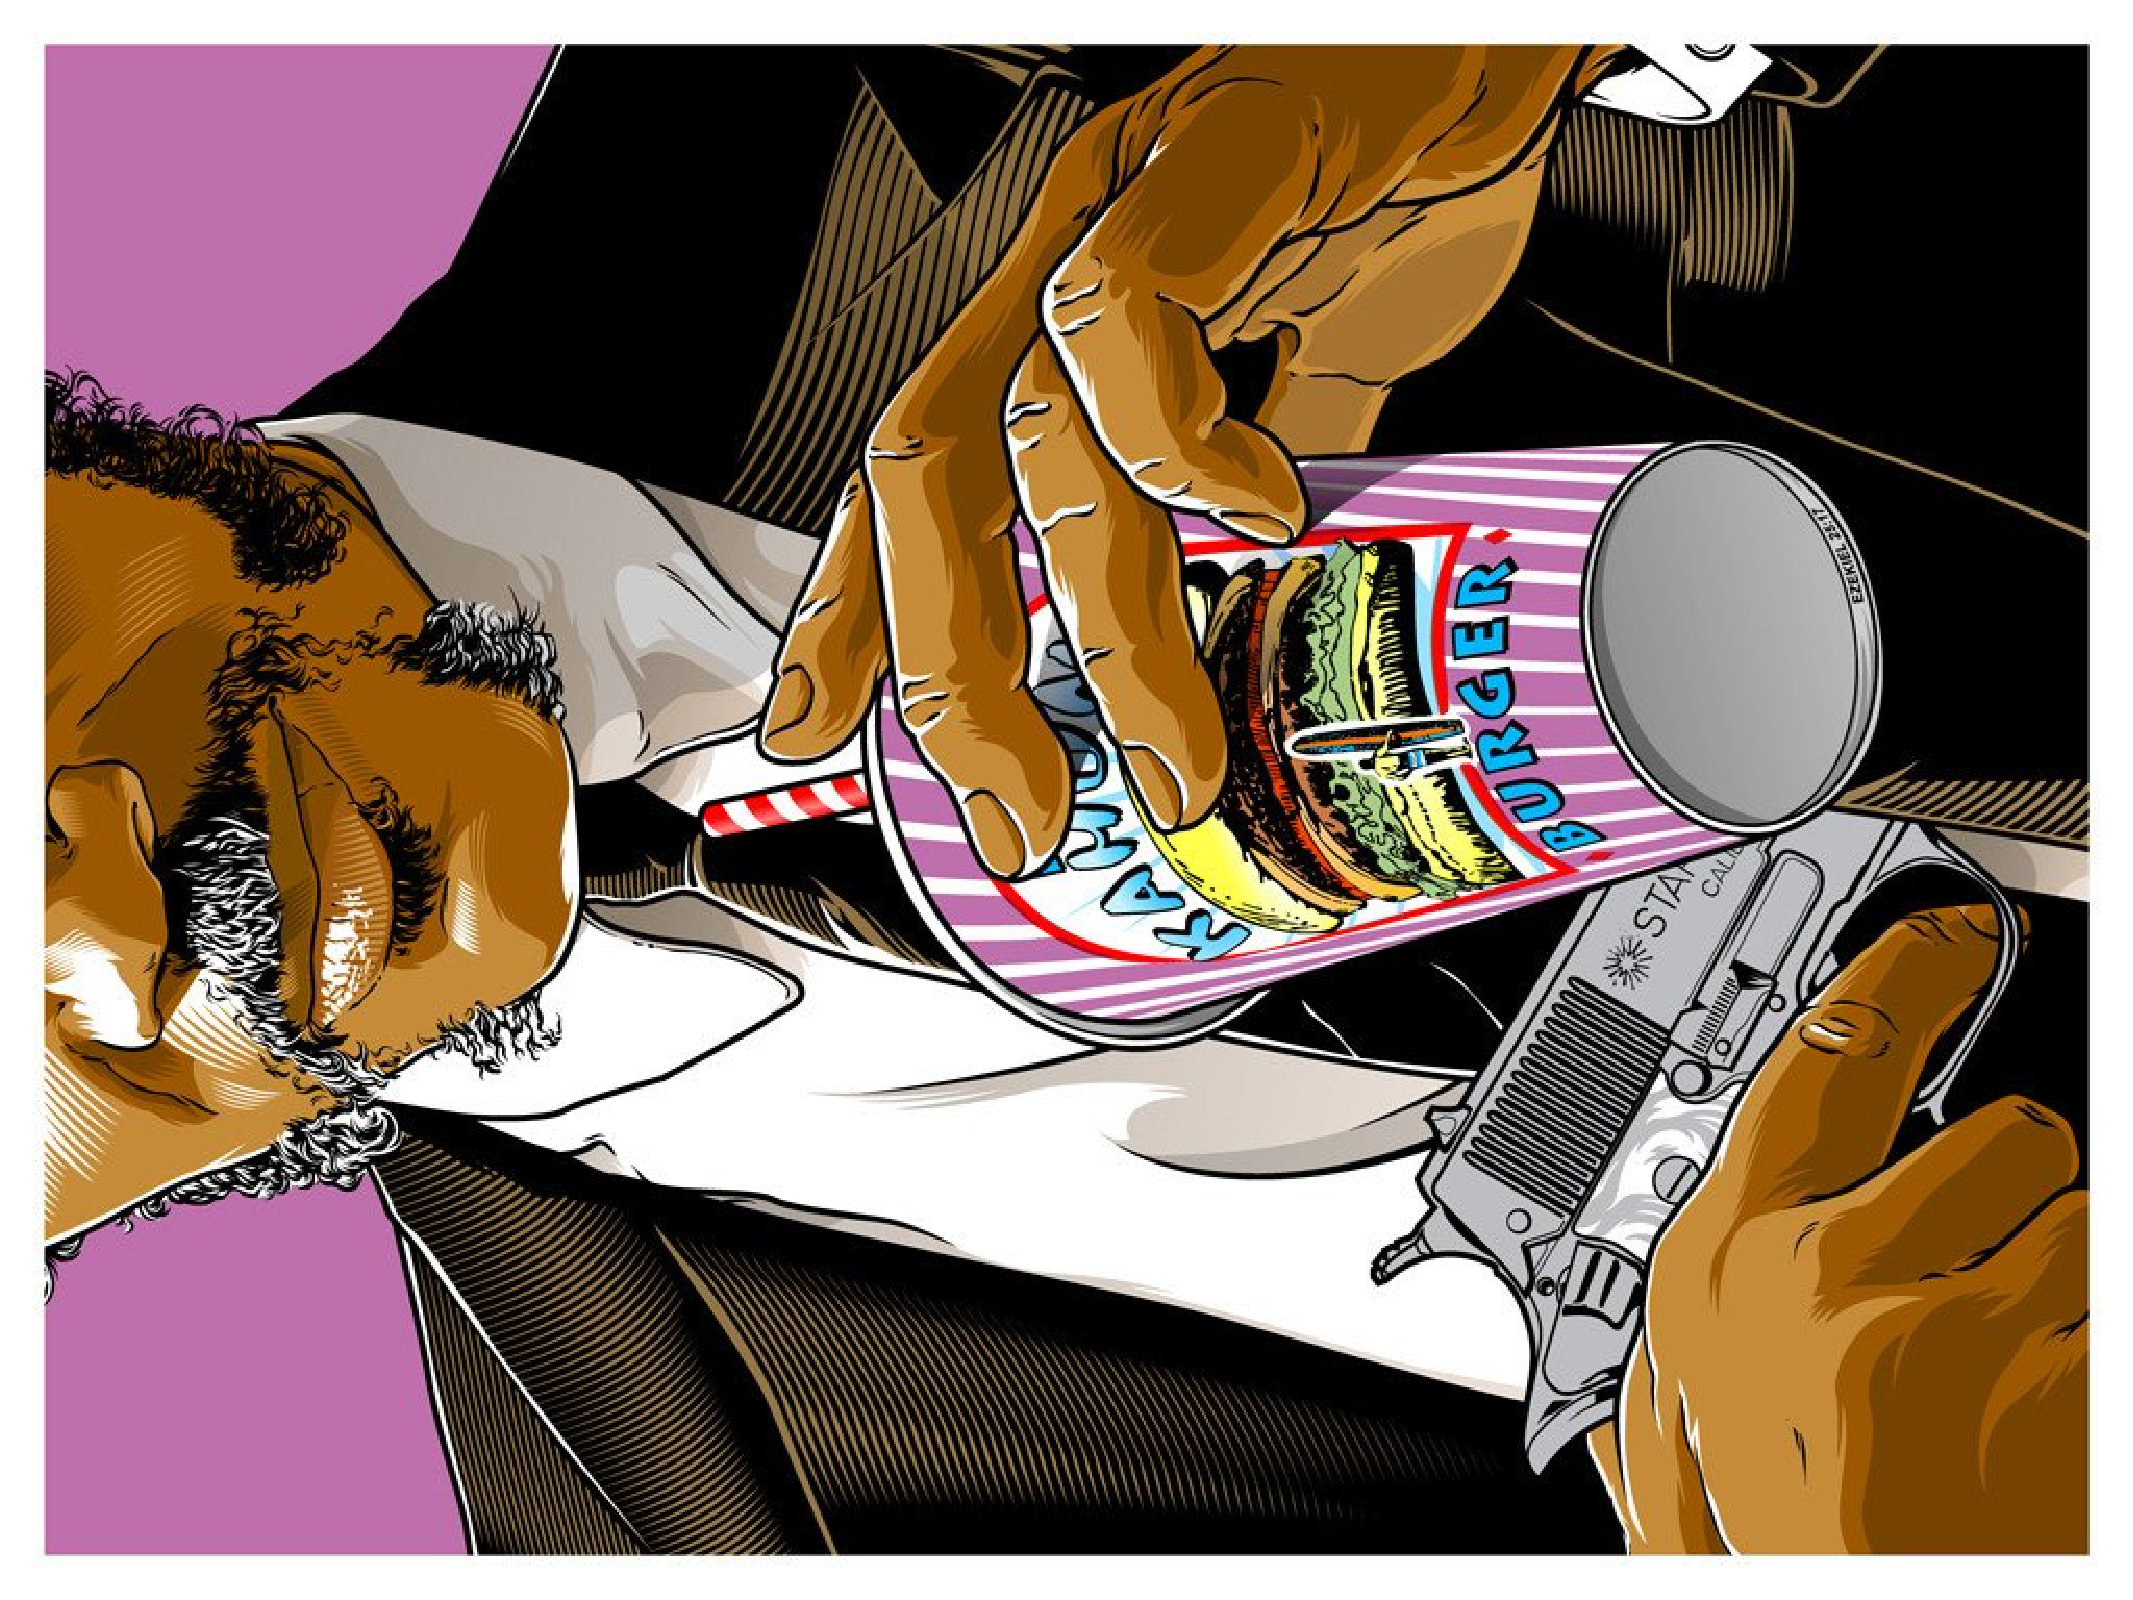
\includegraphics[width=7 cm, angle=270]{pop1.pdf}
\end{minipage}
\hfill
\begin{minipage}{0.3\linewidth}
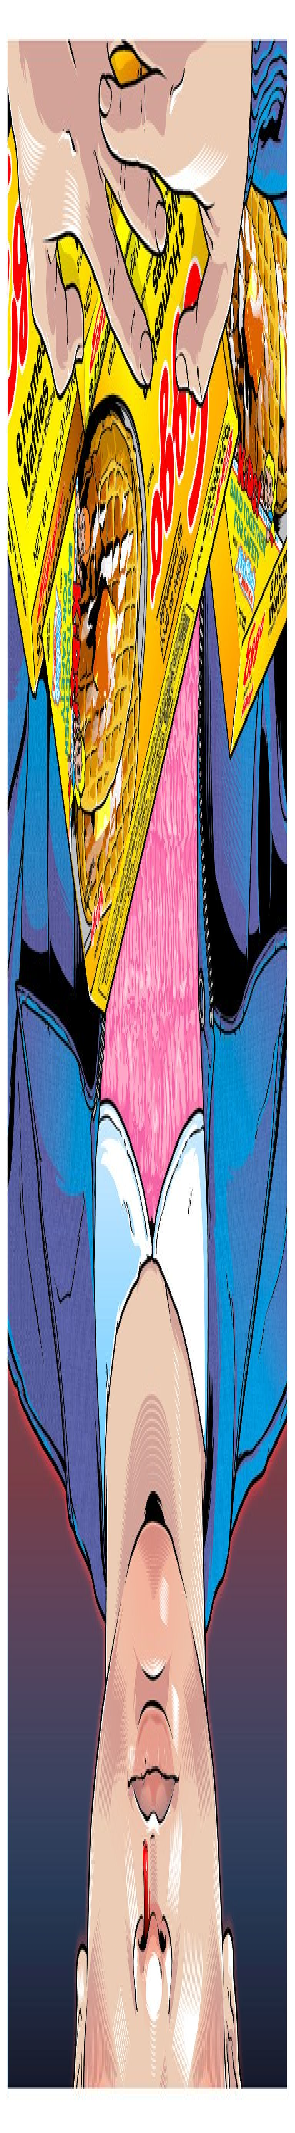
\includegraphics[width=53 mm, height=7 cm, angle=180]{pop2.pdf}
\end{minipage}
\hfill
\begin{minipage}{0.3\linewidth}

\includegraphics[width=52 mm, height=7 cm]{pop3.pdf}
\end{minipage}
\hfill
\begin{minipage}{0.3\linewidth}
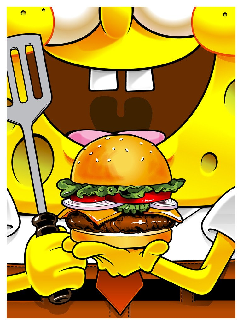
\includegraphics[width=50 mm,height=7 cm]{pop8.pdf}
\end{minipage}
\hfill
\begin{minipage}{0.3\linewidth}
\includegraphics[width=50 mm,height=7 cm]{pop5.pdf}
\end{minipage}
\hfill
\begin{minipage}{0.3\linewidth}
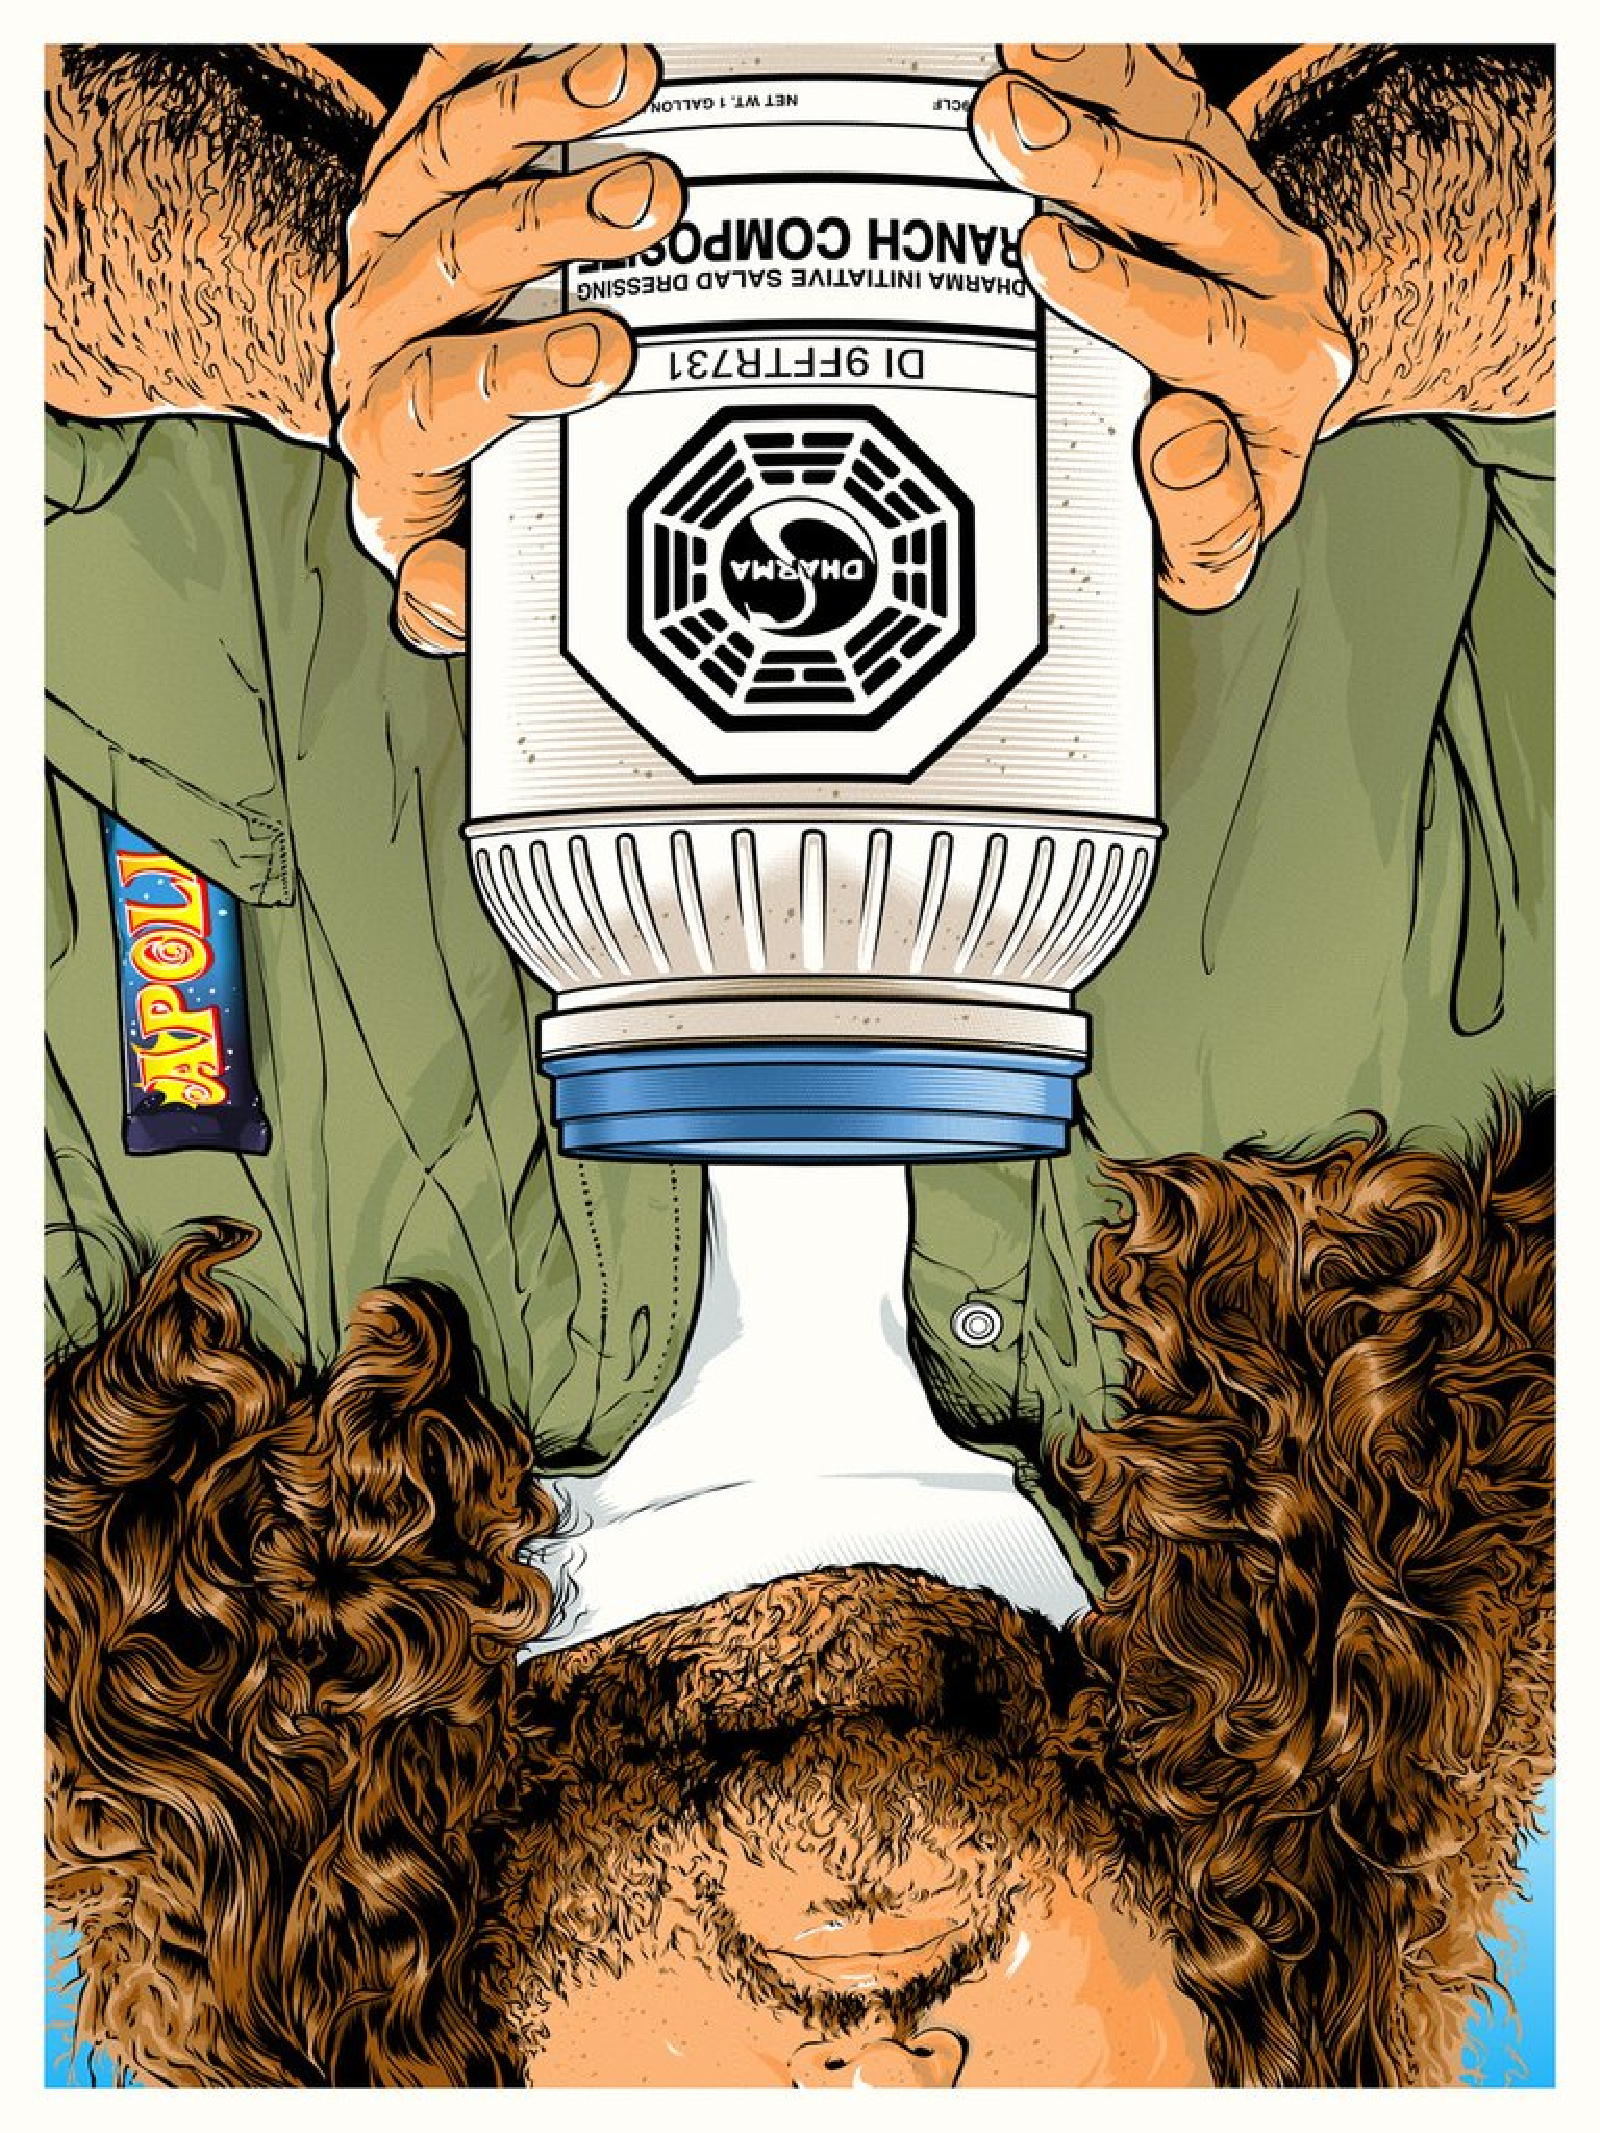
\includegraphics[width=52 mm,height=7 cm, angle= 180]{pop10.pdf}
\end{minipage}
\end{center}
\caption{Что это, поп арт?}
\end{figure}

\end{document}